% !TEX root = ../main.tex
\chapter{Strategic IPO Regulation under Complete and Incomplete Information}
\label{ch:ipo}
\graphicspath{{Chapter_5_IPO/}}

In this chapter, we study the strategic interaction between a financial regulator, responsible for balancing market growth and investor protection, and an issuing firm preparing for an initial public offering (IPO). The regulator prescribes an enforcement tolerance level $\varepsilon$, which bounds the budget by which the firm can window-dress its fundamental feature vector into a presented feature vector while jointly choosing the presentation and share price. The market consists of $k \ge 2$ heterogeneous investor subpopulations with distinct personal valuation functions over the presented features. While the firm seeks to maximize total capital raised, the regulator aims to maximize social welfare by facilitating capital raising by viable firms while curbing misallocations to non-viable firms. We model this interaction as a Stackelberg screening game with the regulator as the leader and the firm as the follower. We analyze this game under two distinct information structures: the \textit{Decision Problem}, in which the feature-valuation distributions are known to the regulator, and the \textit{Learning Problem}, in which these distributions are unknown. In the Decision Problem, we characterize the structure of the firm's optimal pricing and window-dressing decisions and show, through an example, that the optimal regulatory enforcement level can be attained at an interior point. In the Learning Problem, we show that a regulator using a Gaussian Process Thompson Sampling (GP-TS) algorithm with a Mat\'ern-$5/2$ kernel learns the optimal enforcement policy with a sublinear cumulative regret bound of $\widetilde{\mathcal{O}}(T^{2/3})$.

%======================================================================
\section{Introduction}
\label{sec:intro}
%======================================================================

Initial Public Offerings (IPOs) serve as a crucial mechanism for private companies to raise public capital and foster financial market growth. However, significant information asymmetries exist between issuing firms and prospective retail investors. Issuing firms frequently possess incentives to window-dress or strategically modify their presented financial metrics and business features to project a favorable valuation. To prevent investor exploitation and curb capital misallocation to unviable ventures, financial regulatory bodies mandate reporting standards and audit tolerance. Yet, overly stringent regulatory oversight can impose prohibitive compliance burdens, deterring viable firms from entering the capital market. Finding an optimal balance between market growth and investor protection is therefore a fundamental challenge in regulatory economics.

We model this interaction between a welfare-maximizing regulator and a capital-maximizing issuing firm, where the regulator sets an enforcement tolerance limit $\varepsilon$ that constrains the Euclidean distance by which the firm can window-dress its fundamental feature vector $x$ into a presented feature vector $z$, while jointly choosing the presentation and share price. The market consists of heterogeneous investor subpopulations with distinct personal valuation profiles over presented features. The firm seeks to maximize the total capital raised, whereas the regulator seeks to maximize social welfare by facilitating capital raising by viable firms while curbing misallocations to non-viable firms. We formulate this interaction as a Stackelberg screening game, with the regulator as the leader and the issuing firm as the follower.


\subsection{Contributions}

We analyze this regulatory game under two distinct information paradigms: the \emph{Decision Problem} (where feature-valuation distributions are known to the regulator) and the \emph{Learning Problem} (where distributions are unobserved and must be learned through online market interactions).

For the Decision Problem, we prove that for any fixed enforcement level $\varepsilon$, the firm's optimal presentation and pricing strategy reduces to solving $2^k-1$ constrained convex optimization subproblems corresponding to candidate buyer subsets. We further show that expected social welfare need not be monotone in enforcement tolerance. In particular, an overly strict regime ($\varepsilon=0$) can prevent viable firms with low perceived valuations at their baseline features from raising sufficient capital, whereas an overly lax regime ($\varepsilon=\infty$) can enable non-viable firms to mislead investors. An intermediate enforcement level can therefore allow viable firms with low perceived valuations to improve their market prospects while limiting the ability of non-viable firms to mislead investors.


For the Learning Problem, the regulator must learn the optimal enforcement tolerance over a finite time horizon $T$ in a continuous-armed bandit setting. Under market distributions with smooth probability density function with compact support, we show that the expected social welfare function resides in the Reproducing Kernel Hilbert Space (RKHS) associated with a Mat\'ern-$\tfrac{5}{2}$ kernel. Consequently, employing the established Gaussian Process Thompson Sampling (GP-TS) algorithm guarantees a sublinear cumulative regret of $\widetilde{\mathcal{O}}(T^{2/3})$, proving that optimal regulatory oversight can be learned efficiently online.


\subsection{Related Work}

This chapter contributes to the literature on strategic decision making and regulatory policy, bridging strategic feature modification, market segmentation, IPO pricing, and online bandit learning.

\textit{Strategic Feature Modification and Information Design.} Strategic feature modification is studied in~\cite{hardt2016strategic,perdomo2020performative,krishnaswamy2021classification,singh2025strategic,singh2026linear} in screening games where agents modify features or withhold data under decision rules, while information design~\cite{kamenica2011bayesian,bergemann2019information} explores strategic disclosure. While our prior work~\cite{singh2026linear} studied strategic feature revelation where verifiable features are selectively withheld, here the issuing firm actively manipulates (window-dresses) continuous features within a regulatory Euclidean ball.

\textit{Market Segmentation and IPO Pricing.} Classical market segmentation~\cite{bergemann2015limits} studies price discrimination across buyer groups. In our model, although the firm posts a single uniform price, internal subpopulation valuations are used to strategically target investor groups via feature presentation. Traditional IPO literature~\cite{rock1986why,ritter2002review} tracks investor surplus and firm capital under market frictions and information asymmetries; we evaluate analogous welfare and capital objectives, but with an issuing firm that strategically window-dresses features under regulatory enforcement limits.

\textit{Online Continuum-Armed and GP Bandits.} Online bandit literature~\cite{bubeck2011xarmed,flaxman2005online,srinivas2010gp,russo2014learning,chowdhury2017kernelized,vakili2021information,rasmussen2006gaussian} establishes regret bounds under regularity (RKHS) conditions. In our learning setup, we show that market distributions with smooth probability density functions over compact support satisfy these regularity conditions, guaranteeing the $\widetilde{\mathcal{O}}(T^{2/3})$ regret bound. This chapter is derived from our manuscript~\cite{singh2026ipo_journal}. To the best of our knowledge, the problem of regulating strategic window dressing under heterogeneous market valuations across decision and online bandit settings has not been previously studied, and was first explored in our work~\cite{singh2026ipo_journal}.







%======================================================================
\section{Problem Formulation}
\label{sec:model}
%======================================================================

We consider a financial market consisting of a regulator, an issuing firm preparing for an initial public offering (IPO), and a population of prospective retail investors. We model the interaction between the regulator and the issuing firm as a Stackelberg screening game, with the regulator acting as the leader and the issuing firm as the follower. Let $\mathcal{X} \subset \mathbb{R}^d$ be a compact, convex feature space representing fundamental business and financial attributes of the firm, and let $X$ be a random variable defined on $\mathcal{X}$.\index{Initial Public Offering (IPO)|textbf}\index{Strategic window dressing|textbf} The total investor population $\mathcal{N}$ is partitioned into $k \ge 2$ heterogeneous investor subpopulations $\{N_j\}_{j=1}^k$ of random sizes such that $\sum_{j=1}^k N_j = \mathcal{N}$. Each subpopulation $j \in \{1, \dots, k\}$ possesses a bounded, concave valuation function $V_j(z)$ over presented features $z \in \mathcal{X}$. The true stock valuation $Y(X)$ is a random variable given by $Y(X) = V_j(X)$ with probability $\gamma_j(X)$, where $\sum_{j=1}^k \gamma_j(X) = 1$ for all $X \in \mathcal{X}$.


Let $\mathcal{R} := [0, \infty)$ denote the domain of enforcement tolerance levels available to the regulator. Given an enforcement level $\varepsilon \in \mathcal{R}$, the firm's feasible presentation space is bounded within an $\varepsilon$-ball around its true feature vector, $\mathcal{F}_Z(x, \varepsilon) := \{z \in \mathcal{X} : \|x - z\|_2 \le \varepsilon\}$, while its pricing space is $\mathcal{F}_P := \mathbb{R}_+$.\index{Regulatory enforcement tolerance|textbf}\index{Feasible presentation space|textbf} A strategy profile $(\varepsilon, \mathcal{Z}, \mathcal{P})$ maps each feature-enforcement pair $(x, \varepsilon) \in \mathcal{X} \times \mathcal{R}$ to a presentation choice $\mathcal{Z}(x, \varepsilon) \in \mathcal{F}_Z(x, \varepsilon)$ and a posted price $\mathcal{P}(x, \varepsilon) \in \mathcal{F}_P$.

The issuing firm offers a total share supply of $S = \eta \mathcal{N}$, where $\eta \in (0,1]$ represents the supply ratio. Given a presented feature $Z = \mathcal{Z}(X, \varepsilon)$ and posted price $P = \mathcal{P}(X, \varepsilon)$, investors in subpopulation $j$ purchase a share if and only if their personal valuation satisfies $V_j(Z) \ge P$. The aggregate market demand is given by $D(Z, P, \{N_j\}) = \sum_{j=1}^k N_j \mathbf{1}\{V_j(Z) \ge P\}$. Because total supply is capped at $\eta \mathcal{N}$, in the event of demand oversubscription, shares are allocated uniformly among interested buyers. The actual traded volume is given by $Q(Z, P, \{N_j\}, \varepsilon) := \min\{\eta \mathcal{N},\, D(Z, P, \{N_j\})\}$. Total capital raised by the firm and surplus realized by investors are $\Pi_F = P \cdot Q$ and $\Pi_I = (Y(X) - P) \cdot Q$ respectively.\index{Firm capital raised|textbf}\index{Investor valuation profiles|textbf} The realized per-capita social welfare is defined as
\begin{equation}\label{eqn:social_welfare_def}\index{Social welfare|textbf}
W(X, Y, \{N_j\}, \varepsilon; Z, P) := \frac{\Pi_F + \Pi_I}{\mathcal{N}} = \frac{Q(Z, P, \{N_j\}, \varepsilon)\, Y(X)}{\mathcal{N}}.
\end{equation}

The sequence of events in the market proceeds chronologically as follows
\begin{enumerate}[(i)]
    \item \textit{Regulatory Commitment:} The regulator publicly commits to an enforcement tolerance limit $\varepsilon \in \mathcal{R}$.
    \item \textit{Nature's Move:} Nature samples the firm's true feature $X \sim P_X$, subpopulation sizes $\{N_j\}_{j=1}^k$, and valuation realization $Y(X) = V_j(X)$ with probability $\gamma_j(X)$.
    \item \textit{Firm Strategy:} The firm observes baseline feature $X$ and regulatory limit $\varepsilon$, choosing an optimal presentation $Z = \mathcal{Z}(X, \varepsilon) \in \mathcal{F}_Z(X, \varepsilon)$ and price $P = \mathcal{P}(X, \varepsilon) \in \mathcal{F}_P$.
    \item \textit{Market Clearing \& Welfare:} Investors evaluate $V_j(Z)$ and buy if $V_j(Z) \ge P$. Traded volume $Q = \min\{\eta \mathcal{N}, D\}$ yields firm revenue $\Pi_F$ and investor surplus $\Pi_I$, generating realized social welfare $W$.
\end{enumerate}

We examine this formulation under two distinct regulatory information structures: the \emph{Decision Problem} and the \emph{Learning Problem}.

\subsection{Decision Problem}

In the Decision Problem, the subpopulation valuation functions $\{V_j(x)\}_{j=1}^k$ and the joint probability distribution of $(X, Y, \{N_j\})$ are common knowledge. The regulator knows the joint distribution but not the realized instance $(X, Y, \{N_j\})$, whereas the firm observes its realized baseline feature $X=x$.

For any regulatory enforcement action $\varepsilon \in \mathcal{R}$, the firm selects a presentation and pricing strategy to maximize its expected capital raised at realization $X=x$. This \emph{best response} strategy solves

\begin{equation}
\label{eq:firm_br}
\begin{aligned}
&\bigl(\mathcal{Z}^*(x, \varepsilon),\, \mathcal{P}^*(x, \varepsilon)\bigr) \\
&\quad \in \arg\max_{z \in \mathcal{F}_Z(x, \varepsilon),\, p \ge 0} \mathbb{E}_{\{N_j\}}\bigl[\Pi_F(z, p, \{N_j\}, \varepsilon)\bigr].
\end{aligned}
\end{equation}

The regulator seeks to maximize overall expected social welfare. Anticipating the firm's optimal best response $(\mathcal{Z}^*, \mathcal{P}^*)$ for any enforcement tolerance $\varepsilon$, the regulator solves the Stackelberg optimization problem

\begin{equation}
\label{eq:reg_opt}
\begin{aligned}
\varepsilon^* \in \arg\max_{\varepsilon \in \mathcal{R}} \mathbb{E}_{X,\{N_j\},Y}\Bigl[ &W\bigl(X, Y, \{N_j\}, \varepsilon; \\
&\mathcal{Z}^*(X, \varepsilon), \mathcal{P}^*(X, \varepsilon)\bigr)\Bigr].
\end{aligned}
\end{equation}
The resulting strategy tuple $(\varepsilon^*, \mathcal{Z}^*, \mathcal{P}^*)$ constitutes the \emph{Stackelberg equilibrium} of the game.

Let
\begin{equation}
\mathcal{W}(\varepsilon) := \mathbb{E}_{X,\{N_j\},Y}\Bigl[ W\bigl(X, Y, \{N_j\}, \varepsilon; \mathcal{Z}^*(X, \varepsilon), \mathcal{P}^*(X, \varepsilon)\bigr) \Bigr]
\end{equation}
denote the expected social welfare objective function in~\eqref{eq:reg_opt}. To guarantee that $\mathcal{W}(\varepsilon)$ exhibits regular structural properties, we impose the following regularity condition on the market distribution.


\begin{assumption}[Regularity of Market Distribution]
\label{ass:regularity}
The baseline feature vector $X$ has a smooth, bounded probability density function $f_X(x)$ supported on the compact convex domain $\mathcal{X} \subset \mathbb{R}^d$, the discrete valuation types $Y(X) \in \{V_1(X), \dots, V_k(X)\}$ are governed by smooth conditional probabilities $\gamma_j(x)$, and the resulting expected social welfare function $\mathcal{W}(\varepsilon)$ belongs to the RKHS $\mathcal{H}_k([0, \varepsilon_{\max}])$.
\end{assumption}

\begin{remark}[Continuous Density on the Subpopulation Simplex]
\label{rem:simplex}
For tractability, we model the realized subpopulation sizes $(N_1,\dots,N_k)$ by first drawing $(\pi_1,\dots,\pi_k)$ from a continuous distribution over the positive orthant $\mathbb{R}_+^k$ and then setting
\[
N_j = \frac{\pi_j}{\sum_{i=1}^k \pi_i}\mathcal{N},
\qquad j=1,\dots,k,
\]
so that $\sum_{j=1}^k N_j=\mathcal{N}$.
\end{remark}

\subsection{Learning Problem}

In the Learning Problem, the underlying joint distribution of $(X, Y)$ is unknown to the regulator. To preserve analytical tractability, we consider $k=2$ subpopulations with deterministic, equal subpopulation sizes $N_j = \mathcal{N}/2$ almost surely. The concave valuation functions $\{V_j\}_{j=1}^k$ remain common knowledge. The firm knows the marginal distribution of $X$ and observes its realized feature $X_t$ at each round $t$, whereas the regulator must learn the optimal enforcement tolerance $\varepsilon^*$ through repeated market interactions over a finite horizon $T$. Each round consists of the regulator prescribing tolerance $\varepsilon_t$, the firm choosing best response $(\mathcal{Z}_t^*, \mathcal{P}_t^*)$, and the regulator observing the realized social welfare $W_t$.

A \emph{learning algorithm} for the regulator is a sequence of decision rules $\mathcal{A} = \{\mathcal{A}_t\}_{t=1}^T$, where $\mathcal{A}_t : \mathcal{H}_{t-1} \to \mathcal{R}$ maps historical interactions $\mathcal{H}_{t-1} = \{(\varepsilon_\tau, W_\tau)\}_{\tau=1}^{t-1}$ to enforcement level $\varepsilon_t$. The performance of algorithm $\mathcal{A}$ over horizon $T$ is evaluated by its cumulative pseudo-regret:

\begin{equation}
\label{eq:pseudo_regret}
R_T := \sum_{t=1}^T \bigl(\mathcal{W}(\varepsilon^*) - \mathcal{W}(\varepsilon_t)\bigr),
\end{equation}
and its realized regret:
\begin{equation}
\label{eq:regret}
\operatorname{Reg}_{\text{real}}(T) := R_T - \sum_{t=1}^T \xi_t,
\end{equation}
where $\xi_t = W_t - \mathcal{W}(\varepsilon_t)$ is the zero-mean observation noise. A learning algorithm $\mathcal{A}$ achieves \emph{sublinear pseudo-regret} if $R_T = o(T)$.

% Applied Fix: Decoupled RKHS membership from smooth density assumption.

%======================================================================
\section{Decision Problem}
\label{sec:decision}
%======================================================================

In this section, we derive structural results characterizing the Stackelberg equilibrium strategy profile $(\varepsilon^*, \mathcal{Z}^*, \mathcal{P}^*)$ under complete information. We establish that finding the firm's optimal response reduces to a finite set of tractable convex optimization subproblems, and show how the regulator optimizes social welfare over the enforcement domain.

\subsection{Firm's Optimal Strategy}

We first characterize the firm's optimal pricing strategy for any given presentation feature $z \in \mathcal{X}$.

\begin{lemma}
\label{lem:pricing}
For a fixed baseline feature $x \in \mathcal{X}$, regulatory enforcement tolerance $\varepsilon \in \mathcal{R}$, and chosen presentation feature $z \in \mathcal{F}_Z(x, \varepsilon)$, the firm's optimal non-negative pricing strategy satisfies $p^*(z) \in \{0\} \cup \{V_j(z) : V_j(z) \ge 0\}$. If all investor valuations are strictly negative ($V_j(z) < 0$ for all $j$), no trade occurs and the firm earns zero capital.
\end{lemma}
\begin{proof}
The proof is given in Section~\ref{sec:proofs_ch5} (Proof~\ref{proof:lem_pricing}).
\end{proof}

Leveraging this structural property of the optimal price, we now characterize the firm's joint presentation and pricing strategy by targeting candidate buyer subpopulations.

\begin{theorem}
\label{thm:firm_opt}
Assume that the subpopulation valuation functions $V_j(z)$ are concave for all $j \in \{1, \dots, k\}$. For any baseline feature $x \in \mathcal{X}$ and enforcement tolerance $\varepsilon \in \mathcal{R}$, the firm's optimal presentation strategy $\mathcal{Z}^*(x, \varepsilon)$ is determined by solving at most $2^k - 1$ constrained convex optimization subproblems (corresponding to non-empty candidate buyer subsets). For fixed small $k$, this yields an exact and tractable reduction to convex programming.
\end{theorem}
\begin{proof} The proof is given in Section~\ref{sec:proofs_ch5} (Proof~\ref{proof:thm_firm_opt}).
\end{proof}

\subsection{Regulator's Optimization and Social Welfare Smoothness}

To determine the optimal enforcement tolerance $\varepsilon^*$, the regulator must anticipate the firm's best-response policy $(\mathcal{Z}^*(X, \varepsilon), \mathcal{P}^*(X, \varepsilon))$ characterized by Theorem~\ref{thm:firm_opt}. We first establish structural properties of the resulting expected social welfare function $\mathcal{W}(\varepsilon)$.

First, we show that social welfare saturates beyond a finite enforcement threshold, effectively compactifying the relevant domain.

\begin{proposition}
\label{prop:saturation}
For the regulatory enforcement domain $\mathcal{R} = [0, \infty)$, expected social welfare $\mathcal{W}(\varepsilon)$ becomes constant for all $\varepsilon$ beyond a finite saturation threshold $\varepsilon_{\max} < \infty$. Consequently, optimizing $\mathcal{W}(\varepsilon)$ over $\mathcal{R}$ is equivalent to optimizing over the compact domain $[0, \varepsilon_{\max}]$.
\end{proposition}
\begin{proof}
The proof is given in Section~\ref{sec:proofs_ch5} (Proof~\ref{proof:prop_saturation}).
\end{proof}

Having established that the effective enforcement domain is compact, we characterize the regulator's optimization problem over expected social welfare $\mathcal{W}(\varepsilon)$.

% \paragraph{Smoothness of Expected Social Welfare.}\phantomsection\label{thm:smoothness}
% Under Assumption~\ref{ass:regularity}, the market distribution admits a smooth probability density function with compact support. When the firm plays its best response $(\mathcal{Z}^*(x, \varepsilon), \mathcal{P}^*(x, \varepsilon))$, the enforcement tolerance $\varepsilon$ enters through the boundary of the feasible presentation set $\mathcal{F}_Z(x, \varepsilon)$, which partitions the feature space into regions where different buyer subsets are targeted. Differentiating the expected social welfare $\mathcal{W}(\varepsilon) = \mathbb{E}_X[W(X, \varepsilon)]$ via Leibniz's rule transfers all derivatives with respect to $\varepsilon$ to boundary evaluations against the smooth feature density. Because the density has compact support and uniformly bounded derivatives of all orders, the expected social welfare function $\mathcal{W}(\varepsilon)$ is infinitely differentiable ($\mathcal{C}^\infty$) on the compact interval $[0, \varepsilon_{\max}]$.

\paragraph{Regulator's Optimization and Tractability}
Anticipating the firm's optimal best-response policy $(\mathcal{Z}^*(X, \varepsilon), \mathcal{P}^*(X, \varepsilon))$ from Theorem~\ref{thm:firm_opt}, the regulator determines the optimal enforcement tolerance by solving:
\begin{equation}
\label{eq:eps_star}
\varepsilon^* \in \arg\max_{\varepsilon \in [0, \varepsilon_{\max}]} \mathcal{W}(\varepsilon).
\end{equation}
Because $\mathcal{W}(\varepsilon)$ is smooth and the domain $[0, \varepsilon_{\max}]$ is compact, finding the global optimum $\varepsilon^*$ reduces to maximizing a continuous, smooth objective over a compact interval. For any specified approximation tolerance $\delta > 0$, compactness guarantees that the domain $[0, \varepsilon_{\max}]$ can be covered by a finite number of $\delta$-balls (or evaluated on a finite grid of mesh size $\delta$), ensuring that $\varepsilon^*$ can be efficiently computed to within tolerance $\delta$ using only finitely many evaluations.


%======================================================================
\subsection{Illustrative Example: Finding optimal regulation for affine valuation functions}
\label{ssec:analytical_proof}
%======================================================================

To characterize optimal regulatory policy, we consider an instance of the IPO problem with $k=2$ investor subpopulations, denoted by $\alpha$ and $\beta$. The market consists of equal population shares ($\pi_\alpha = \pi_\beta = 1/2$), so that $N_\alpha = N_\beta = \mathcal{N}/2$. The feature space $\mathcal{X} \subseteq \mathbb{R}^d$ is convex and compact, with $0$ in its interior. Baseline feature vectors $X \in \mathcal{X}$ are distributed according to a smooth probability density function $f_X(x)$. The personal valuation functions for subpopulations $\alpha$ and $\beta$ are:
\begin{equation}
V_\alpha(z) = w_\alpha^\top z + b_\alpha \quad \text{and} \quad V_\beta(z) = w_\beta^\top z + b_\beta
\end{equation}
respectively. Conditional on baseline realization $X = x$, the true asset value per share $Y \in \mathbb{R}$ realizes as $V_\alpha(x)$ with probability $\gamma(x) \in [0,1]$ and as $V_\beta(x)$ with probability $1 - \gamma(x)$. Furthermore we assume $\eta = 1$, i.e., total number of shares available is $\mathcal{N}$. Let
\begin{equation}
\mu(x) := \mathbb{E}[Y \mid X = x] = \gamma(x) V_\alpha(x) + \bigl(1 - \gamma(x)\bigr) V_\beta(x).
\end{equation} Given regulatory enforcement tolerance $\varepsilon \in [0, \varepsilon_{\max}]$ and baseline feature realization $x \in \mathcal{X}$, the issuing firm selects a presentation vector $z = x + \Delta \in \mathcal{F}_Z(x, \varepsilon) = \{z \in \mathbb{R}^d : \|\Delta\|_2 \le \varepsilon\}$ and posted price $P \ge 0$. From Theorem~\ref{thm:firm_opt}, the firm identifies its optimal response by maximizing capital raised $\Pi_F = P \cdot Q$ across the $2^2 - 1 = 3$ possibilities:
\begin{enumerate}[(i)]
\item Targeting Subpopulation $\alpha$:
  To maximize the perceived valuation of subpopulation $\alpha$, the firm chooses its manipulation vector with $\Delta_\alpha^* = \varepsilon \frac{w_\alpha}{\|w_\alpha\|_2}$. The optimal posted price is
  \begin{equation}
  P_\alpha^*(x, \varepsilon) = V_\alpha(x + \Delta_\alpha^*) = w_\alpha^\top x + b_\alpha + \varepsilon \|w_\alpha\|_2.
  \end{equation}
  At this price, only subpopulation $\alpha$ purchases shares, yielding traded volume $Q_\alpha = N_\alpha = \mathcal{N}/2$. The firm's private capital raised is:
  \begin{equation}
  \Pi_{F,\alpha}(x, \varepsilon) = \frac{\mathcal{N}}{2}\left(w_\alpha^\top x + b_\alpha + \varepsilon \|w_\alpha\|_2\right).
  \end{equation}
  Investors in subpopulation $\alpha$ earn a profit of $\Pi_{I} = Q_\alpha(Y(x) - P_\alpha^*)$. The realized per-capita social welfare is $\frac{\Pi_{F,\alpha} + \Pi_{I}}{\mathcal{N}} = \frac{Q_\alpha Y(x)}{\mathcal{N}} = \frac{1}{2}Y(x)$ and the expected social welfare is $\mathbb{E}[\frac{\mu(x)}{2}]$.
  
\item Targeting Subpopulation $\beta$: Just as in for targetting subpopilation $\alpha$, the firm sets its manipulation vector with $\Delta_\beta^* = \varepsilon \frac{w_\beta}{\|w_\beta\|_2}$, and posts price
  \begin{equation}
  P_\beta^*(x, \varepsilon) = w_\beta^\top x + b_\beta + \varepsilon \|w_\beta\|_2.
  \end{equation}
  Traded volume is $Q_\beta = N_\beta = \mathcal{N}/2$, and the firm raises capital:
  \begin{equation}
  \Pi_{F,\beta}(x, \varepsilon) = \frac{\mathcal{N}}{2}\left(w_\beta^\top x + b_\beta + \varepsilon \|w_\beta\|_2\right).
  \end{equation}
  Investors in subpopulation $\beta$ earn a profit of $\Pi_{I} = Q_\beta(Y(x) - P_\beta^*)$, yielding conditional expected per-capita social welfare $\mathbb{E}[\frac{\mu(x)}{2}]$.
  
\item Targeting Both Subpopulations: Since the entire stock of IPO has to be sold ($Q_{\alpha\beta} = N_\alpha + N_\beta = \mathcal{N}$), both subpopulations must be presented with the same manipulated feature vector $z = x + \Delta \in \mathcal{F}_Z(x, \varepsilon)$. The market-clearing price that induces both groups to purchase is constrained by the lower of their two valuations under the common presentation. Thus, the optimal common price is obtained by solving the max--min program:
  \begin{equation}
  \label{eq:p_alphabeta_simple}
  P_{\alpha\beta}^*(x, \varepsilon) = \max_{\|\Delta\|_2 \le \varepsilon} \min\bigl\{V_\alpha(x + \Delta),\, V_\beta(x + \Delta)\bigr\}.
  \end{equation}
  The firm's capital raised is
  \begin{equation}
  \Pi_{F,\alpha\beta}(x, \varepsilon) = \mathcal{N} P_{\alpha\beta}^*(x, \varepsilon),
  \end{equation}
  and the investors' profit is $\Pi_{I} = \mathcal{N}(Y(x) - P_{\alpha\beta}^*)$. The conditional expected per-capita social welfare is $\frac{\Pi_F + \Pi_{I}}{\mathcal{N}} = \mu(x)$.
\end{enumerate}

\begin{remark}[Optimal Common Presentation for Affine Valuations]
\label{rem:joint_manipulation}
For affine valuations $V_j(z) = w_j^\top z + b_j$, the max--min problem \eqref{eq:p_alphabeta_simple} seeks a common manipulation $\Delta$ satisfying $\|\Delta\|_2 \le \varepsilon$ that maximizes $\min\{w_\alpha^\top(x+\Delta) + b_\alpha,\, w_\beta^\top(x+\Delta) + b_\beta\}$. Posing this as a standard convex program yields the optimal manipulation direction parameterized by a Lagrange multiplier $\lambda \in [0,1]$:
\begin{equation}
\Delta_{\alpha\beta}^* = \varepsilon \frac{\lambda w_\alpha + (1-\lambda) w_\beta}{\|\lambda w_\alpha + (1-\lambda) w_\beta\|_2}.
\end{equation}
When the firm balances both groups ($\lambda = 1/2$), the common manipulation aligns with the angular bisector $\frac{w_\alpha + w_\beta}{\|w_\alpha + w_\beta\|_2}$. Under equal sensitivity norms $\|w_\alpha\|_2 = \|w_\beta\|_2 = w_0$, if $w_\alpha \perp w_\beta$ (orthogonal preferences), the common presentation yields a per-group manipulation gain of $\frac{\varepsilon w_0}{\sqrt{2}}$, reflecting the geometric cost of a shared presentation compared to the separate single-group gain $\varepsilon w_0$.
\end{remark}
The firm's optimal targeting rule partitions the fundamental feature space $\mathbb{R}^d$ into three mutually disjoint decision regions:
\begin{align}
\mathcal{R}_\alpha(\varepsilon) &\triangleq \bigl\{x \in \mathbb{R}^d : \Pi_{F,\alpha}(x,\varepsilon) > \max(\Pi_{F,\beta}(x,\varepsilon),\, \Pi_{F,\alpha\beta}(x,\varepsilon))\bigr\}, \\
\mathcal{R}_\beta(\varepsilon) &\triangleq \bigl\{x \in \mathbb{R}^d : \Pi_{F,\beta}(x,\varepsilon) > \max(\Pi_{F,\alpha}(x,\varepsilon),\, \Pi_{F,\alpha\beta}(x,\varepsilon))\bigr\}, \\
\mathcal{R}_{\alpha\beta}(\varepsilon) &\triangleq \bigl\{x \in \mathbb{R}^d : \Pi_{F,\alpha\beta}(x,\varepsilon) \ge \max(\Pi_{F,\alpha}(x,\varepsilon),\, \Pi_{F,\beta}(x,\varepsilon))\bigr\}.
\end{align}

The expected social welfare is given by:
\begin{equation}
\label{eq:welfare_simplified}
\begin{aligned}
\mathcal{W}(\varepsilon) &= \int_{\mathcal{R}_\alpha(\varepsilon)} \frac{1}{2} \mu(x) f_X(x) \, dx + \int_{\mathcal{R}_\beta(\varepsilon)} \frac{1}{2} \mu(x) f_X(x) \, dx + \int_{\mathcal{R}_{\alpha\beta}(\varepsilon)} 1 \cdot \mu(x) f_X(x) \, dx\\
&= \frac{1}{2} \mathbb{E}[\mu(X)] + \frac{1}{2} \int_{\mathcal{R}_{\alpha\beta}(\varepsilon)} \mu(x) f_X(x) \, dx.
\end{aligned}
\end{equation}
The regulation level $\varepsilon$ influences social welfare exclusively through the set $\mathcal{R}_{\alpha\beta}(\varepsilon) = \bigl\{x \in \mathbb{R}^d : \Pi_{F,\alpha\beta}(x,\varepsilon) \ge \max(\Pi_{F,\alpha}(x,\varepsilon),\, \Pi_{F,\beta}(x,\varepsilon))\bigr\}$. We now characterise this set into two sectors.
\begin{enumerate}[(a)]
\item When $P_\alpha^*(x, \varepsilon) \ge P_\beta^*(x, \varepsilon)$, we have $P_{\alpha\beta}^* = P_\beta^*$. The firm prefers serving both groups over targeting group $\alpha$ alone if and only if $\Pi_{F,\alpha\beta} \ge \Pi_{F,\alpha} \iff \mathcal{N} P_\beta^* \ge \frac{\mathcal{N}}{2} P_\alpha^*$, which yields the linear half-space condition
  \begin{equation}
  \label{eq:halfspace_alpha}
  \left(w_\beta^\top x + b_\beta + \varepsilon \|w_\beta\|_2\right) - \frac{1}{2}\left(w_\alpha^\top x + b_\alpha + \varepsilon \|w_\alpha\|_2\right) = a_\alpha^\top x - c_\alpha + \rho_\alpha \varepsilon \ge 0,
  \end{equation}
  where
  \begin{equation}
  \label{eq:params_alpha}
  a_\alpha := w_\beta - \frac{1}{2}w_\alpha \in \mathbb{R}^d, \qquad c_\alpha := \frac{1}{2}b_\alpha - b_\beta \in \mathbb{R}, \qquad \rho_\alpha := \|w_\beta\|_2 - \frac{1}{2}\|w_\alpha\|_2 \in \mathbb{R}.
  \end{equation}

\item When $P_\beta^*(x, \varepsilon) > P_\alpha^*(x, \varepsilon)$, we have $P_{\alpha\beta}^* = P_\alpha^*$. The condition $\Pi_{F,\alpha\beta} \ge \Pi_{F,\beta} \iff \mathcal{N} P_\alpha^* \ge \frac{\mathcal{N}}{2} P_\beta^*$ similarly gives
  \begin{equation}
  \label{eq:halfspace_beta}
  \left(w_\alpha^\top x + b_\alpha + \varepsilon \|w_\alpha\|_2\right) - \frac{1}{2}\left(w_\beta^\top x + b_\beta + \varepsilon \|w_\beta\|_2\right) = a_\beta^\top x - c_\beta + \rho_\beta \varepsilon \ge 0,
  \end{equation}
  where
  \begin{equation}
  \label{eq:params_beta}
  a_\beta := w_\alpha - \frac{1}{2}w_\beta \in \mathbb{R}^d, \qquad c_\beta := \frac{1}{2}b_\beta - b_\alpha \in \mathbb{R}, \qquad \rho_\beta := \|w_\alpha\|_2 - \frac{1}{2}\|w_\beta\|_2 \in \mathbb{R}.
  \end{equation}
\end{enumerate}
Thus $\mathcal{R}_{\alpha\beta}(\varepsilon)$ partitions into two disjoint boundary sectors $\mathcal{R}_{\alpha\beta}(\varepsilon) = \mathcal{R}_{\alpha\beta,\alpha}(\varepsilon) \cup \mathcal{R}_{\alpha\beta,\beta}(\varepsilon)$, where
\begin{align}
\mathcal{R}_{\alpha\beta,\alpha}(\varepsilon) &:= \left\{x \in \mathbb{R}^d : a_\alpha^\top x \ge c_\alpha - \rho_\alpha \varepsilon\right\} \cap C_\alpha, \\
\mathcal{R}_{\alpha\beta,\beta}(\varepsilon) &:= \left\{x \in \mathbb{R}^d : a_\beta^\top x \ge c_\beta - \rho_\beta \varepsilon\right\} \cap C_\beta,
\end{align}
with price-ordering sectors $C_\alpha := \{x \in \mathbb{R}^d : P_\alpha^*(x, \varepsilon) \ge P_\beta^*(x, \varepsilon)\}$ and $C_\beta := \{x \in \mathbb{R}^d : P_\beta^*(x, \varepsilon) > P_\alpha^*(x, \varepsilon)\}$. Under equal biases $b_\alpha = b_\beta = b_0$ and equal sensitivity norms $\|w_\alpha\|_2 = \|w_\beta\|_2 = w_0$, these sectors simplify to $C_\alpha = \{x : (w_\alpha - w_\beta)^\top x \ge 0\}$ and $C_\beta = \{x : (w_\alpha - w_\beta)^\top x < 0\}$, which are static and form a partition of the feature space $\mathcal{X}$.

Let $S_j := a_j^\top X \in \mathbb{R}$ denote the scalar random variable with marginal probability density function $f_{S_j}(s)$. Defining the sector-restricted conditional expected valuation as $\bar{\mu}_j(s) := \mathbb{E}[\mu(X)\mathbf{1}_{C_j}(X) \mid S_j = s]$, the Law of Iterated Expectations yields
\begin{equation}
\label{eq:lie_disintegration_step}
\int_{\mathcal{R}_{\alpha\beta, j}(\varepsilon)} \mu(x) f_X(x) \, dx = \mathbb{E}\Bigl[\mu(X) \mathbf{1}_{C_j}(X) \mathbf{1}_{\{S_j \ge c_j - \rho_j \varepsilon\}}\Bigr] = \int_{c_j - \rho_j \varepsilon}^\infty \bar{\mu}_j(s) f_{S_j}(s) \, ds.
\end{equation}
Because $C_\alpha \cap C_\beta = \emptyset$ and $C_\alpha \cup C_\beta = \mathcal{X}$, upon full saturation when $c_j - \rho_j \varepsilon \le s_{\min, j}$ for both sectors, $\sum_{j \in \{\alpha, \beta\}} \int_{-\infty}^\infty \bar{\mu}_j(s) f_{S_j}(s) \, ds = \mathbb{E}[\mu(X)(\mathbf{1}_{C_\alpha}(X) + \mathbf{1}_{C_\beta}(X))] = \mathbb{E}[\mu(X)]$, cleanly verifying the full-sale limit without double counting. Substituting into~\eqref{eq:welfare_simplified}, we obtain expected social welfare as
\begin{equation}
\label{eq:welfare_1d_disintegration}
\mathcal{W}(\varepsilon) = \frac{1}{2} \mathbb{E}[\mu(X)] + \frac{1}{2} \sum_{j \in \{\alpha, \beta\}} \int_{c_j - \rho_j \varepsilon}^{\infty} \bar{\mu}_j(s) f_{S_j}(s) \, ds.
\end{equation}
Since $\varepsilon$ appears solely in the lower limit of integration, the Fundamental Theorem of Calculus yields
\begin{align}
\label{eq:w_prime_full}
\mathcal{W}'(\varepsilon) &= \frac{1}{2} \sum_{j \in \{\alpha, \beta\}} \rho_j \cdot \bar{\mu}_j(c_j - \rho_j \varepsilon) \cdot f_{S_j}(c_j - \rho_j \varepsilon), \\
\label{eq:w_double_prime_full}
\mathcal{W}''(\varepsilon) &= -\frac{1}{2} \sum_{j \in \{\alpha, \beta\}} \rho_j^2 \left[ \bar{\mu}_j'(c_j - \rho_j \varepsilon) f_{S_j}(c_j - \rho_j \varepsilon) + \bar{\mu}_j(c_j - \rho_j \varepsilon) f_{S_j}'(c_j - \rho_j \varepsilon) \right].
\end{align}


\paragraph{Simplification under Equal Biases and Equal Weight Norms}
To characterize the qualitative behavior of optimal regulation, we assume equal baseline biases $b_\alpha = b_\beta = b_0 \in \mathbb{R}$ and equal sensitivity norms $\|w_\alpha\|_2 = \|w_\beta\|_2 = w_0 > 0$ with $w_\alpha \neq w_\beta$. This assumption implies $c_\alpha = c_\beta = c := -\frac{1}{2} b_0$ and $\rho_\alpha = \rho_\beta = \rho := \frac{1}{2} w_0 > 0$. Recall that the feature space $\mathcal{X}$ is convex and compact with $0 \in \mathrm{int}(\mathcal{X})$ and $a_j \neq 0$, therefore each random variable $S_j = a_j^\top X$ has bounded support $[s_{\min, j}, s_{\max, j}]$, where $s_{\min, j} := \min_{x \in \mathcal{X}} a_j^\top x < 0$ and $s_{\max, j} := \max_{x \in \mathcal{X}} a_j^\top x > 0$. For each boundary sector, the lower integration limit $c - \rho \varepsilon$ sweeps across the support of $S_j$ as $\varepsilon$ increases. By Proposition~\ref{prop:saturation}, expected social welfare saturates once $c - \rho \varepsilon \le s_{\min, j}$ for all $j \in \{\alpha, \beta\}$, thus $\varepsilon_{\max} = \max_{j\in\{\alpha,\beta\}} ((c - s_{\min, j})/\rho) < \infty$. Therefore, the expected welfare and its derivatives simplify to
\begin{align}
\mathcal{W}(\varepsilon) &= \frac{1}{2}\mathbb{E}[\mu(X)] + \frac{1}{2}\sum_{j\in\{\alpha,\beta\}} \int_{c - \rho \varepsilon}^{s_{\max, j}} \bar{\mu}_j(s) f_{S_j}(s)\,ds, \\
\mathcal{W}'(\varepsilon) &= \frac{\rho}{2} \sum_{j\in\{\alpha,\beta\}} \bar{\mu}_j(c - \rho \varepsilon) f_{S_j}(c - \rho \varepsilon), \label{eq:w_prime_reduced} \\
\mathcal{W}''(\varepsilon) &= -\frac{\rho^2}{2} \sum_{j\in\{\alpha,\beta\}} \left[ \bar{\mu}_j'(c - \rho \varepsilon) f_{S_j}(c - \rho \varepsilon) + \bar{\mu}_j(c - \rho \varepsilon) f_{S_j}'(c - \rho \varepsilon) \right].
\end{align}

We now establish a sufficient condition for $\mathcal{W}(\varepsilon)$ to be optimal at an interior point.

\begin{proposition}[Non-monotonicity of the welfare function]
\label{prop:interior_optimality}
Let baseline feature space $\mathcal{X} \subset \mathbb{R}^d$ be compact and convex with $0 \in \mathrm{int}(\mathcal{X})$. Assume equal biases $b_\alpha = b_\beta = b_0$, equal sensitivity norms $\|w_\alpha\|_2 = \|w_\beta\|_2 = w_0 > 0$, and marginal densities satisfy $f_{S_j}(s) > 0$ on $(s_{\min, j}, s_{\max, j})$. If the conditional expected valuation functions $\bar{\mu}_j(s) := \mathbb{E}[\mu(X) \mid S_j = s]$ satisfy
\begin{enumerate}[(i)]
    \item Strict monotonicity: $\bar{\mu}_j'(s) > 0$ for all $s \in [s_{\min, j}, s_{\max, j}]$ and each $j \in \{\alpha, \beta\}$,
    \item Viability at baseline cutoff: $\bar{\mu}_j(c) > 0$ for each $j \in \{\alpha, \beta\}$, where $c = -\frac{1}{2}b_0$,
    \item Non-viability of lowest baseline features: $\bar{\mu}_j(s_{\min, j}) < 0$ for each $j \in \{\alpha, \beta\}$,
\end{enumerate}
then the optimal regulatory enforcement policy $\varepsilon^*$ lies strictly in the interior of the enforcement domain, $\varepsilon^* \in (0, \varepsilon_{\max})$, satisfying $\mathcal{W}'(\varepsilon^*) = 0$.
\end{proposition}
\begin{proof} The proof is given in Section~\ref{sec:proofs_ch5} (Proof~\ref{proof:prop_interior_optimality}).
\end{proof}

\paragraph{Verification of Non-Emptiness}
To confirm that the sufficient conditions of Proposition~\ref{prop:interior_optimality} are non-empty, consider a 2D market instance with equal baseline biases $b_\alpha = b_\beta = 1$ (so $c = -\frac{1}{2}$) and orthogonal investor sensitivity vectors $w_\alpha = (2, 0)^\top$ and $w_\beta = (0, 2)^\top$, so that $\|w_\alpha\|_2 = \|w_\beta\|_2 = 2$ and $\rho = 1$. The investor valuations are $V_\alpha(x) = 2x_1 + 1$ and $V_\beta(x) = 2x_2 + 1$. Assuming equal mixture probabilities $\gamma_\alpha = \gamma_\beta = 1/2$, the true fundamental expected valuation is the valid convex combination $\mu(x) = \frac{1}{2}V_\alpha(x) + \frac{1}{2}V_\beta(x) = x_1 + x_2 + 1$. The vectors $a_\alpha = (-1, 2)^\top$ and $a_\beta = (2, -1)^\top$ define the scores $S_\alpha = -X_1 + 2X_2$ and $S_\beta = 2X_1 - X_2$, which satisfy $S_\alpha + S_\beta = X_1 + X_2$. We define the feature space as the compact convex domain $\mathcal{X} = \{x \in \mathbb{R}^2 : -3 \le -x_1 + 2x_2 \le 3 \text{ and } -3 \le 2x_1 - x_2 \le 3\}$ with uniform distribution $X \sim U(\mathcal{X})$. Because this linear transformation maps $\mathcal{X}$ bijectively onto the product domain $[-3, 3]^2$, the variables $S_\alpha$ and $S_\beta$ are independent uniform random variables on $[-3, 3]$ with support bounds $s_{\min} = -3 < 0 < 3 = s_{\max}$ and saturation threshold $\varepsilon_{\max} = c - s_{\min} = 2.5$. Within each symmetric sector, $\bar{\mu}_j(s) = \frac{1}{2}(s + \mathbb{E}[S_{j'}]) + \frac{1}{2} = \frac{1}{2}s + \frac{1}{2}$. This directly satisfies all three conditions: (i) $\bar{\mu}_j'(s) = 1/2 > 0$, (ii) $\bar{\mu}_j(c) = \bar{\mu}_j(-0.5) = 0.25 > 0$, and (iii) $\bar{\mu}_j(-3) = -1 < 0$. Solving $\mathcal{W}'(\varepsilon^*) = 0$ yields the unique interior optimal enforcement policy $\varepsilon^* = 2.0 \in (0, 2.5)$, with $\mathcal{W}''(\varepsilon^*) < 0$, confirming strict concavity and global interior maximality.


% Applied Fix: Corrected joint presentation price to max-min formulation and recalculated conditional means.

We extend beyond the linear setting by conducting Monte Carlo simulations ($5{,}000$ independent market realizations per enforcement level $\varepsilon$, $\pm 1$ standard error bands)\coderef{subsec:code_ipo_decision} with logistic valuation functions:
\begin{equation}
  V_j(z) = \sigma(u_j + v_j z), \quad \sigma(s) = \frac{1}{1+e^{-s}}.
\end{equation}
We fix $N_1=N_2=50$, $\eta=1$, $X\sim U[-1,1]$, and Group~1 parameters at $u_1=0$, $v_1=+4$ throughout. Group~2 parameters are varied across two parameter families:

\begin{enumerate}
  \item[(i)] \textit{$\gamma$-Sweep (Panels~(a) and~(b), Figure~\ref{fig:decision_sim}):} $u_2=0$ fixed; $v_2 \in \{-8,-6,-4,-2,+2\}$.
  \item[(ii)] \textit{$\delta$-Sweep (Panels~(c) and~(d), Figure~\ref{fig:decision_sim}):} $v_2=-4$ fixed; $u_2 \in \{-4,-2,0,+2,+4\}$.
\end{enumerate}

Figure~\ref{fig:decision_sim} displays the simulation results, illustrating the non-monotonic trajectory of expected social welfare alongside expected firm capital in representative instances, as well as the asymptotic saturation of curves as $\varepsilon$ increases across all configurations, empirically corroborating our theoretical findings.

\begin{figure}[t]
\centering
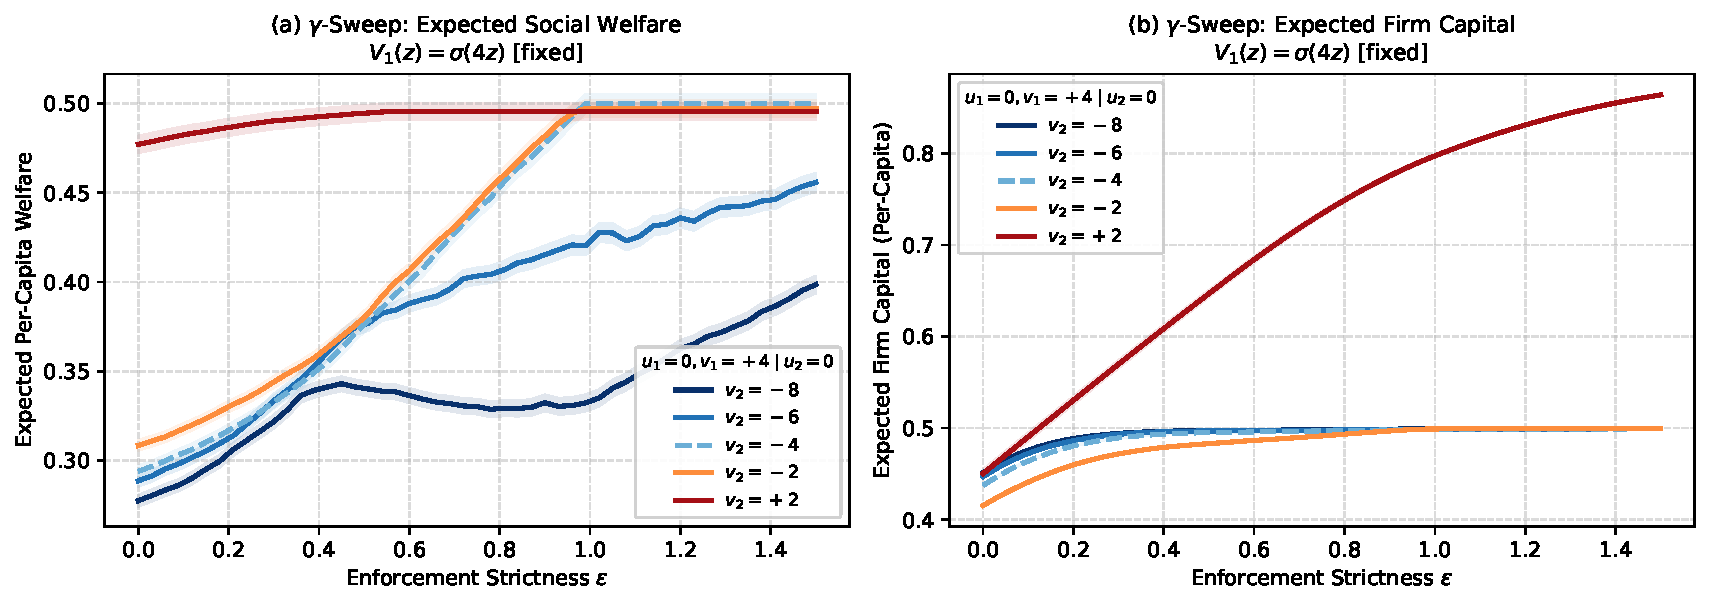
\includegraphics[width=\textwidth]{figures/decision_sim_results.pdf}
\caption{Decision problem simulation across the $\gamma$-sweep and $\delta$-sweep.}
\label{fig:decision_sim}
\end{figure}

% !TEX root = ../../main.tex
%======================================================================
\section{Learning Problem}
\label{sec:learning}
%======================================================================

In this section, we examine the regulatory setting under incomplete information, where the underlying joint market distribution $(X, Y, \{N_j\})$ is unknown to the regulator. We formulate the regulator's search for optimal enforcement tolerance $\varepsilon^*$ as an online continuum-armed bandit problem.\index{Online regulatory learning|textbf} We apply the well-established framework of Gaussian Process Thompson Sampling (GP-TS)~\cite{chowdhury2017kernelized} to analyze learning performance in our strategic IPO regulation setting.

At each round $t = 1, \dots, T$, the regulator selects an enforcement tolerance $\varepsilon_t \in [0, \varepsilon_{\max}]$ and subsequently observes the realized social welfare $W_t = \mathcal{W}(\varepsilon_t) + \xi_t$, where $\xi_t = W_t - \mathcal{W}(\varepsilon_t)$ represents zero-mean observation noise arising from market realization randomness.

Under Assumption~\ref{ass:regularity}, the expected social welfare function $\mathcal{W}(\varepsilon)$ is $C^{\infty}$ over the compact domain $[0, \varepsilon_{\max}]$. Because $C^{\infty}([0, \varepsilon_{\max}])$ is densely embedded in the Sobolev space $H^3([0, \varepsilon_{\max}])$, which is norm-equivalent to the Reproducing Kernel Hilbert Space (RKHS) $\mathcal{H}_k$ of the Mat\'ern-$5/2$ kernel (for comprehensive background on Mat\'ern kernels and RKHS properties, see, e.g., \cite{rasmussen2006gaussian, chowdhury2017kernelized}):
\begin{equation}
\label{eq:matern}
\begin{aligned}
k_{5/2}(\varepsilon, \varepsilon')
&= \sigma_0^2 \biggl( 1 + \frac{\sqrt{5}\,|\varepsilon-\varepsilon'|}{l} + \frac{5(\varepsilon-\varepsilon')^2}{3l^2} \biggr) \\
&\quad \times \exp\biggl( -\frac{\sqrt{5}\,|\varepsilon-\varepsilon'|}{l} \biggr),
\end{aligned}
\end{equation}
it follows directly that $\mathcal{W} \in \mathcal{H}_k$ with a bounded RKHS norm $\|\mathcal{W}\|_{\mathcal{H}_k} \le B < \infty$. Here $\sigma_0^2 > 0$ is the signal variance and $l > 0$ is the characteristic length-scale parameter (for detailed information about Matérn kernels and RKHS refer \cite{chowdhury2017kernelized}).

The regulator employs GP-TS (Algorithm~\ref{alg:gpts}) to adaptively select $\varepsilon_t$. By placing a GP prior $\mathcal{GP}(0, k_{5/2})$ over $\mathcal{W}$, the regulator maintains posterior mean $\mu_{t-1}(\cdot)$ and covariance $k_{t-1}(\cdot,\cdot)$ updated via standard Gaussian process regression equations over past history $\mathcal{H}_{t-1} = \{(\varepsilon_\tau, W_\tau)\}_{\tau=1}^{t-1}$:
\begin{equation}
\label{eq:gp_update}
\begin{aligned}
\mu_{t-1}(\varepsilon) &= k_{t-1}(\varepsilon)^\top (K_{t-1} + \sigma^2 I)^{-1} \mathbf{W}_{t-1}, \\
k_{t-1}(\varepsilon, \varepsilon') &= k_{5/2}(\varepsilon, \varepsilon') - k_{t-1}(\varepsilon)^\top (K_{t-1} + \sigma^2 I)^{-1} k_{t-1}(\varepsilon'),
\end{aligned}
\end{equation}
where $k_{t-1}(\varepsilon) = [k_{5/2}(\varepsilon_1, \varepsilon), \dots, k_{5/2}(\varepsilon_{t-1}, \varepsilon)]^\top$, $K_{t-1}$ is the $(t-1) \times (t-1)$ kernel matrix with entries $[K_{t-1}]_{ij} = k_{5/2}(\varepsilon_i, \varepsilon_j)$, and $\mathbf{W}_{t-1} = [W_1, \dots, W_{t-1}]^\top$.

\begin{algorithm}[t]\index{Gaussian Process Thompson Sampling!for IPO regulation|textbf}
\caption{Gaussian Process Thompson Sampling (GP-TS) for IPO Regulation}
\label{alg:gpts}
\begin{algorithmic}[1]
\State \textbf{Input:} Mat\'ern-$5/2$ kernel $k_{5/2}(\cdot,\cdot)$, GP prior $\mathcal{GP}(0, k_{5/2})$, domain $[0, \varepsilon_{\max}]$, horizon $T$, noise variance $\sigma^2$, confidence $\delta \in (0,1)$.
\For{$t = 1, 2, \dots, T$}
  \State Set inflation factor $v_t = B + R\sqrt{2(\gamma_{t-1} + 1 + \log(2/\delta))}$ \citep{chowdhury2017kernelized}.
  \State Compute GP posterior mean $\mu_{t-1}(\varepsilon)$ and covariance $k_{t-1}(\varepsilon,\varepsilon')$ using~\eqref{eq:gp_update} based on history $\mathcal{H}_{t-1}$.
  \State Sample function candidate $\widetilde{\mathcal{W}}_t \sim \mathcal{GP}(\mu_{t-1},\, v_t^2 k_{t-1})$.
  \State Select regulatory enforcement tolerance $\varepsilon_t \in \arg\max_{\varepsilon \in \mathcal{D}_t} \widetilde{\mathcal{W}}_t(\varepsilon)$ over round-$t$ net $\mathcal{D}_t \subset [0, \varepsilon_{\max}]$.
  \State Apply $\varepsilon_t$ to the market and observe realized social welfare $W_t$.
  \State Update interaction history $\mathcal{H}_t = \mathcal{H}_{t-1} \cup \{(\varepsilon_t, W_t)\}$ and update posterior parameters.
\EndFor
\end{algorithmic}
\end{algorithm}

Applying the established regret analysis of GP-TS for kernelized continuum-armed bandits~\cite{chowdhury2017kernelized} directly specializes the general sublinear regret guarantee to our strategic IPO regulation problem.

\begin{theorem}[Regret Guarantee for IPO enforcement tolerance]
\label{thm:regret}
Under Assumption~\ref{ass:regularity}, if the regulator employs GP-TS (Algorithm~\ref{alg:gpts}) with the Mat\'ern-$5/2$ kernel $k_{5/2}$, the cumulative regret $R_T = \sum_{t=1}^T \bigl(\mathcal{W}(\varepsilon^*) - \mathcal{W}(\varepsilon_t)\bigr)$ is bounded with probability at least $1-\delta$ by
\begin{equation}
\label{eq:rt_bound}
R_T = \widetilde{\mathcal{O}}\!\left(T^{2/3}\right).
\end{equation}
\end{theorem}

\begin{proof} The proof is given in Section~\ref{sec:proofs_ch5} (Proof~\ref{proof:thm_regret}).
\end{proof}

To empirically validate the learning performance of the GP-TS algorithm in regulatory enforcement design, we simulate the continuous bandit problem across independent trials.\coderef{subsec:code_ipo_learning} We consider an underlying market environment with $k=2$ investor subpopulations of equal size ($N_1 = N_2 = 50$, $\mathcal{N} = 100$, $\eta = 1$), baseline feature $X \sim U[-1/3, 1/3]$, and linear valuation profiles $V_1(z) = 1+3z$ and $V_2(z) = 1-3z$. The firm's true valuation $Y(X)$ takes value in $\{V_1(X), V_2(X)\}$ according to probabilities $\gamma_1(X)$ and $\gamma_2(X)$, inducing observation noise in realized social welfare $W_t$; we evaluate learning performance under two noise conditions: low noise ($\sigma = 0.05$) and high noise ($\sigma = 0.25$). At each round $t$, after selecting enforcement strictness $\varepsilon_t \in [0, 1.2]$, the regulator observes realized social welfare $W_t$.

The cumulative regret trajectories ($R_T$) displayed in Figure~\ref{fig:learning} exhibit sublinear growth bounded by the theoretical $\widetilde{\mathcal{O}}(T^{2/3})$ rate established in Theorem~\ref{thm:regret} across both noise levels (shaded bands denote $\pm 1$ standard error across $40$ independent trials).

\begin{figure}[t]
\centering
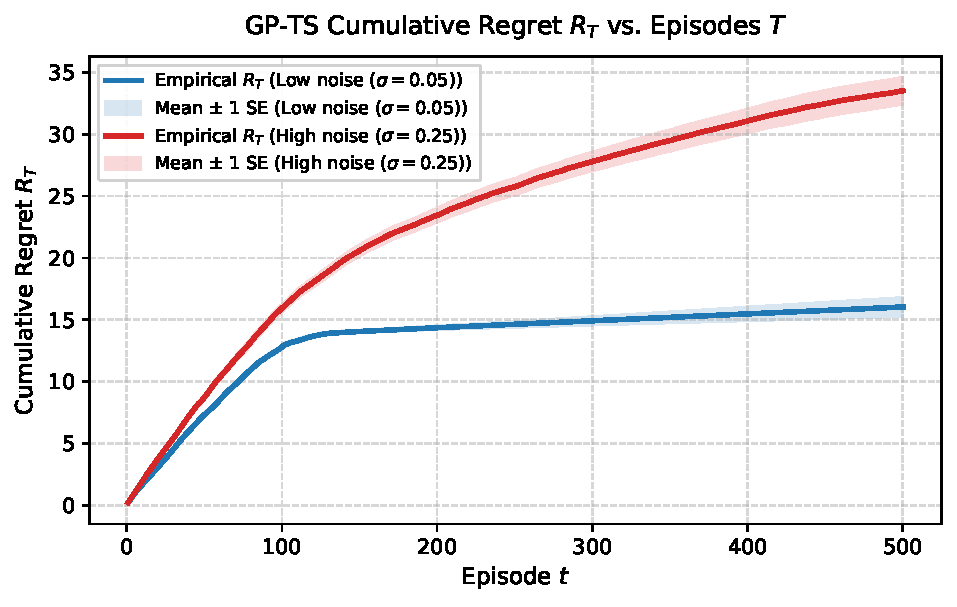
\includegraphics[width=0.72\columnwidth]{figures/learning_results.pdf}
\caption{Cumulative regret $R_T$ of GP-TS online regulatory learning under low ($\sigma=0.05$) and high ($\sigma=0.25$) noise (solid curves show mean cumulative regret, shaded bands indicate $\pm 1$ standard error across $40$ trials).}
\label{fig:learning}
\end{figure}


%======================================================================
\section{Conclusion, Limitations, and Future Work}
\label{sec:conclusion}
%======================================================================



In this chapter, we presented a game-theoretic framework for strategic IPO regulation, modeling the interaction between a welfare-maximizing financial regulator and a capital-maximizing issuing firm capable of feature window-dressing under a regulatory enforcement budget $\varepsilon$.

Under the \emph{Decision Problem}, we established that the issuing firm's optimal presentation and pricing strategy reduces to solving $2^k-1$ constrained convex optimization subproblems corresponding to candidate buyer subpopulations. We showed that expected social welfare need not be monotone in regulatory tolerance: overly rigid enforcement can prevent viable firms with low perceived valuations at their baseline features from raising sufficient capital, while excessively lax enforcement can enable non-viable firms to mislead investors. An intermediate enforcement level can therefore allow viable firms to improve their market prospects while limiting the ability of non-viable firms to mislead investors.




Under the \emph{Learning Problem}, we modeled online regulatory search as a continuum-armed bandit problem. We established that when the market distribution of $(X,Y,\{N_j\})$ has compact support and admits a smooth probability density function with bounded density and derivatives, 
the expected welfare function belongs to the Reproducing Kernel Hilbert Space (RKHS) of a Matérn-$5/2$ kernel. Using the established Gaussian Process Thompson Sampling (GP-TS) algorithm, we obtained a provably sublinear cumulative regret of $\widetilde{\mathcal{O}}(T^{2/3})$.

A key limitation of our formulation is the assumption of naive face-value investors who purchase based directly on their personal valuation of the presented features. Promising directions for future work include considering more sophisticated investors and richer dynamics in which the regulator and the issuing firm adaptively learn the market distribution and respond strategically to one another over time.


%======================================================================
\section{Proofs and Supporting Results}
\label{sec:proofs_ch5}
%======================================================================

This section provides the proofs for the theoretical results presented in this chapter.

\subsection{Proofs for the Decision Problem}

In this subsection, we provide the proofs of the theoretical results for the decision problem.

\phantomsection
We now provide the proof of Lemma~\ref{lem:pricing}.
\begin{proof}[Proof of Lemma~\ref{lem:pricing}: Optimal Pricing Strategy]\label{app:proof_lem_pricing}\label{proof:lem_pricing}
For any fixed presentation feature $z$, the valuation of each investor subpopulation $j$ is $V_j(z)$. The aggregate market demand $D(z, p, \{N_j\}) = \sum_{j=1}^k N_j \mathbf{1}\{V_j(z) \ge p\}$ is a piecewise-constant step function that is non-increasing in price $p \ge 0$, with jump discontinuities occurring exclusively at price points $p \in \{V_1(z), \dots, V_k(z)\}$. If all investor valuations are strictly negative ($\max_j V_j(z) < 0$), no buyer enters at any non-negative price $p \ge 0$, yielding zero demand and zero capital (the no-trade option). If at least one subpopulation has non-negative valuation, the expected traded volume $\mathbb{E}_{\{N_j\}}[Q(z, p, \{N_j\}, \varepsilon)]$ is constant on each interval $(v_m, v_{m+1}]$, where $v_m$ and $v_{m+1}$ are adjacent values in the sorted set $\{0\} \cup \{V_j(z) : V_j(z) \ge 0\}$. The firm's expected capital raised $p \cdot \mathbb{E}_{\{N_j\}}[Q]$ is strictly increasing on $(v_m, v_{m+1})$, so the supremum on any such interval is attained at its right endpoint. Hence, the optimal non-negative price satisfies $p^*(z) \in \{0\} \cup \{V_j(z) : V_j(z) \ge 0\}$.
\end{proof}

\phantomsection
We now provide the proof of Theorem~\ref{thm:firm_opt}.
\begin{proof}[Proof of Theorem~\ref{thm:firm_opt}: Firm's Optimal Presentation Strategy]\label{app:proof_thm_firm_opt}\label{proof:thm_firm_opt}
For any target subset $S \subseteq \{1, \dots, k\}$, setting price $p_S(z) = \min_{j \in S} V_j(z)$ ensures participation of at least all groups in $S$, establishing a lower bound $\Pi_F^{(S)}(z) \le \Pi_F(z,\min_{j \in S}V_j)$ given by
\begin{equation}
\Pi_F^{(S)}(z) = \Bigl(\min_{j \in S} V_j(z)\Bigr) \cdot \mathbb{E}_{\{N_j\}}\Bigl[\min\Bigl\{\eta \mathcal{N},\, \sum_{j \in S} N_j\Bigr\}\Bigr].
\end{equation}
At the optimal strategy $(z^*, p^*)$, Lemma~\ref{lem:pricing} guarantees $p^* = V_{m^*}(z^*)$. For the true buyer set $S^* = \{j : V_j(z^*) \ge p^*\}$, market demand equals $\sum_{j \in S^*} N_j$ exactly, making the lower bound tight, i.e., $\Pi_F^{(S^*)}(z^*) = \Pi_F(z^*, p^*)$. Because $\Pi_F^{(S)}(z) \le \max_{z,p} \Pi_F(z, p)$ for all $S$ and equality is achieved at $(S^*, z^*)$, maximizing these lower bounds over all $S$ and $z$ recovers the exact global maximum. Since each $\Pi_F^{(S)}(z)$ is concave in $z$ (as the pointwise minimum of concave functions), evaluating $\max_z \Pi_F^{(S)}(z)$ over $z \in \mathcal{F}_Z(x, \varepsilon)$ defines a constrained convex optimization subproblem. Therefore, solving these $2^k - 1$ convex subproblems and selecting the maximum yields the global optimum.
\end{proof}

\phantomsection
We now provide the proof of Proposition~\ref{prop:saturation}.
\begin{proof}[Proof of Proposition~\ref{prop:saturation}: Welfare Saturation Threshold]\label{app:proof_prop_saturation}\label{proof:prop_saturation}
Consider the unconstrained presentation problem where the firm faces no regulatory budget constraints ($\varepsilon = \infty$), yielding optimal presentation $z_{\infty}^*(x) = \arg\max_{z \in \mathcal{X}} \max_S \Pi_F^{(S)}(z, \infty)$. The minimal regulatory budget required to accommodate this unconstrained move is $\varepsilon_{\max}(x) = \|x - z_{\infty}^*(x)\|_2$. Because the baseline feature space $\mathcal{X}$ is a compact subset of $\mathbb{R}^d$, the continuous distance mapping $\varepsilon_{\max}(x)$ achieves a finite supremum $\varepsilon_{\max} = \sup_{x \in \mathcal{X}} \varepsilon_{\max}(x) < \infty$. For any tolerance $\varepsilon \ge \varepsilon_{\max}$, the unconstrained optimal presentation $z_{\infty}^*(x)$ lies within the feasible space $\mathcal{F}_Z(x, \varepsilon)$ for every realization $x \in \mathcal{X}$. Consequently, the firm's optimal presentation and pricing strategies $(\mathcal{Z}^*(x, \varepsilon), \mathcal{P}^*(x, \varepsilon))$ and expected social welfare $\mathcal{W}(\varepsilon)$ remain constant for all $\varepsilon \ge \varepsilon_{\max}$, restricting the optimization domain to $[0, \varepsilon_{\max}]$ without loss of generality.
\end{proof}

\phantomsection
We now provide the proof of Proposition~\ref{prop:interior_optimality}.
\begin{proof}[Proof of Proposition~\ref{prop:interior_optimality}: Non-Monotonicity and Interior Optimality]\label{app:proof_prop_interior_optimality}\label{proof:prop_interior_optimality}
Evaluating $\mathcal{W}'(\varepsilon)$ at $\varepsilon = 0$ yields $\mathcal{W}'(0) = \frac{\rho}{2} [ \bar{\mu}_\alpha(c) f_{S_\alpha}(c) + \bar{\mu}_\beta(c) f_{S_\beta}(c) ]$. Since $\rho > 0$, $f_{S_j}(c) > 0$, and $\bar{\mu}_j(c) > 0$ by condition~(ii), it follows that $\mathcal{W}'(0) > 0$, showing that social welfare strictly increases locally at $\varepsilon = 0$. Next, since $\varepsilon_{\max} = \max_{j\in\{\alpha,\beta\}} ((c - s_{\min,j})/\rho)$, as $\varepsilon \to \varepsilon_{\max}^-$, we have $c - \rho \varepsilon \to s_{\min, j}^+$. Because $\bar{\mu}_j(s_{\min, j}) < 0$ by condition~(iii), $f_{S_j}(s) > 0$ on $(s_{\min, j}, s_{\max, j})$, and $\rho > 0$, taking the left-hand limit yields $\mathcal{W}'(\varepsilon_{\max}^-) < 0$, showing that social welfare strictly decreases locally at $\varepsilon = \varepsilon_{\max}$. Because $\mathcal{W}'(\varepsilon)$ is continuous on the compact interval $[0, \varepsilon_{\max}]$ with $\mathcal{W}'(0) > 0$ and $\mathcal{W}'(\varepsilon_{\max}^-) < 0$, the Intermediate Value Theorem guarantees the existence of an interior stationary point $\varepsilon^* \in (0, \varepsilon_{\max})$ satisfying $\mathcal{W}'(\varepsilon^*) = 0$. Since the boundary points $\varepsilon \in \{0, \varepsilon_{\max}\}$ yield strictly lower welfare than nearby interior points, the global maximum on $[0, \varepsilon_{\max}]$ must be attained at an interior policy $\varepsilon^* \in (0, \varepsilon_{\max})$. Furthermore, condition~(i) ensures strict monotonicity $\bar{\mu}_j'(s) > 0$, guaranteeing the second-order sufficient condition for a maximum, $\mathcal{W}''(\varepsilon^*) = -\frac{\rho^2}{2} \sum_j \bar{\mu}_j'(c - \rho \varepsilon^*) f_{S_j}(c - \rho \varepsilon^*) < 0$.
\end{proof}

\subsection{Proofs for the Learning Problem}

In this subsection, we provide the proof of the regret bound for the regulatory learning problem.

\phantomsection
We now provide the proof of Theorem~\ref{thm:regret}.
\begin{proof}[Proof of Theorem~\ref{thm:regret}: Regret Bound for Regulatory GP-TS]\label{app:proof_thm_regret}\label{proof:thm_regret}
Under Assumption~\ref{ass:regularity}, the expected social welfare function $\mathcal{W}(\varepsilon)$ is smooth on $[0, \varepsilon_{\max}]$ and belongs to the RKHS $\mathcal{H}_k$ of $k_{5/2}$ with bounded norm $\|\mathcal{W}\|_{\mathcal{H}_k} \le B < \infty$. Furthermore, because traded share volume is bounded by total supply $\eta \mathcal{N}$ and valuations are bounded in magnitude by $Y_{\max}$, realized social welfare satisfies the symmetric envelope $|W_t| \le \eta Y_{\max}$. Consequently, the observation noise $\xi_t = W_t - \mathcal{W}(\varepsilon_t)$ is conditionally $R$-sub-Gaussian with $R = \eta Y_{\max}$ by Hoeffding's Lemma.

Applying the GP-TS regret bound of \citet[Theorem 4]{chowdhury2017kernelized} on the 1D compact domain $[0, \varepsilon_{\max}]$, cumulative regret satisfies $R_T = \mathcal{O}\bigl(B\sqrt{T\gamma_T} + \gamma_T\sqrt{T}\bigr)$, where $\gamma_T$ is the maximum information gain for kernel $k_{5/2}$. For the Mat\'ern-$5/2$ kernel on a 1D compact domain ($d=1, \nu=5/2$), the maximum information gain is bounded by $\gamma_T = \widetilde{\mathcal{O}}(T^{\frac{d}{2\nu+d}}) = \widetilde{\mathcal{O}}(T^{1/6})$ \citep{vakili2021information}. Substituting $\gamma_T = \widetilde{\mathcal{O}}(T^{1/6})$ yields the sublinear cumulative regret bound $R_T = \widetilde{\mathcal{O}}(T^{2/3})$.
\end{proof}

% Applied Fix: Added zero-revenue option in subset proof and retained derivative terms in interior-optimality proof.

